\documentclass[12pt]{article}

\usepackage{fancyhdr}
\usepackage{makeidx}
\usepackage[catalan]{babel}
\usepackage{amsfonts}
\usepackage{amssymb}
\usepackage{amsthm}
\usepackage{amsmath}
\usepackage[all]{xy}
%\usepackage[ansinew]{inputenc} %%
\usepackage[utf8]{inputenc}
\usepackage[dvips]{epsfig}
\usepackage{color}
\usepackage{multicol}



%\usepackage[spanish]{babel}
%\usepackage{color}% usar color para las letras
%\usepackage{graphics}
%\usepackage{graphicx}
%\usepackage{amssymb}
%\usepackage{amsfonts}%para poder poner las letras de Reales Complejos etc...
%\usepackage{anysize} % Soporte para el comando \marginsize
%\usepackage[latin1]{inputenc}% permite poner acentos de forma normal

\setlength{\textwidth}{16cm} \setlength{\textheight}{24cm}
\setlength{\oddsidemargin}{-0.3cm} \setlength{\topmargin}{-1.3cm}

%\usepackage{texfonts}
%\marginsize{2cm}{2cm}{2cm}{2cm}
%\newcommand{\ZZ}{\mathbbmss{Z}}
%\usepackage{fancyhdr}
%\renewcommand{\rmdefault}{phv}
%%%%%%%%%%%%%%%%%%%%%%%%%%%%%%%%%%%%%%%%%%%%%%%%%%%%%%%%%%%%%%%%%%%%%%%%
%-- nuevos comandos para facilitar la escritura
\newcommand{\notacio}{\textbf{Notaci{\'o}}\ \ }
\newcommand{\demostracio}{\textbf{Demostraci{\'o}}\ \ }
\newcommand{\propietats}{\textbf{Propietats}\ \ }
\newcommand{\propietat}{\textbf{Propietat}\ \ }
%\newcommand{\exemple}{\textbf{Exemple}\ \ }
\newcommand{\exemples}{\textbf{Exemples}\ \ }
\newcommand{\observacio}{\textbf{Observaci{\'o}}\ \ }
\newcommand{\observacions}{\textbf{Observacions}\ \ }
\newcommand{\solucio}{\textbf{Soluci{\'o}}\ \ }


\newtheorem{definicio}{Definici{\'o}}[subsection]
\newtheorem{teorema}{Teorema}[subsection]
\newtheorem{Teorema}{Teorema}[subsubsection]
\newtheorem{proposicio}{Proposici{\'o}}[subsection]
\newtheorem{lema}{Lema}[subsection]
\newtheorem{corol}{Corol.lari}[subsection]
\newtheorem{exemple}{Exemple}[subsection]
\newtheorem{prob}{Problema}[subsection]


\newcommand{\Z}{\mathbb{Z}}
\newcommand{\R}{\mathbb{R}}
\newcommand{\C}{\mathbb{C}}
\newcommand{\N}{\mathbb{N}}
\newcommand{\U}{\mathcal{U}}
\newcommand{\V}{\mathcal{V}}
\newcommand{\W}{\mathcal{W}}
\newcommand{\sen}{\mathop{\rm sen}\nolimits}

\begin{document}

%\vspace*{7cm}
%\begin{center}
%\textbf{\Huge{C{\`a}lcul II}}
%
%\vspace*{2cm}\textbf{\LARGE{Primer curs}}
%
%\vspace*{2cm}\textbf{\LARGE{Grau en Enginyeria Telem{\`a}tica}}
%\end{center}
%
%\thispagestyle{empty}
%
%\newpage
%

\pagenumbering{arabic}
\pagestyle{fancy}
\fancyhead{}
\fancyhead[RE,RO]{Tema 1. Els nombres complexos}
\fancyfoot[RE,RO]{Autor: Marc Carbonell 2011}


\begin{center}
\section{Tema 1. Els Nombres Complexos}
\end{center}

\parskip =0.3cm
\parindent =0cm
\itemindent=2cm

\subsection{Introducci{\'o}.}

La manera habitual d'introduir el concepte de nombre complex sol ser
indicant que amb els nombres reals no n'hi ha prou, que hi ha certes
equacions de segon grau que no som capa\c{c}os de resoldre nom{\'e}s amb els
nombres reals. Per exemple, l'equaci{\'o}
$$x^{2}+1=0$$
\'{e}s irresoluble en $\R$.\\

Hist{\`o}ricament, els nombres complexos apareixen en el Renaixement i
no precisament per a resoldre equacions de segon grau sin\'{o} quan
volem resoldre equacions de tercer grau.

La f{\'o}rmula de Tartaglia (o de Scipione del Ferro) per a
resoldre l'equaci{\'o}:
$$x^{3}+px+q=0$$
\'{e}s:
$$x=\sqrt[3]{\frac{-q}{2}+\sqrt{\frac{p^{3}}{27}+\frac{q^2}{4}}}
\ +\ \sqrt[3]{\frac{-q}{2}-\sqrt{\frac{p^{3}}{27}+\frac{q^2}{4}}}\
.$$

Si l'aplicam per a resoldre l'equaci{\'o} $\ x^{3}-7x+6=0\ $
obtenim:\\

$$x=\sqrt[3]{-3+\sqrt{\frac{-100}{27}}}\ +\ \sqrt[3]{-3-\sqrt{\frac{-100}{27}}}$$\\

Una soluci{\'o} s'obt\'{e} observant que:

$\left(1+\sqrt{\frac{-4}{3}}\;\right)^{3}=-3+\sqrt{\frac{-100}{27}}$\hspace{1cm}
i tamb{\'e} que \hspace{1cm}$\left(1-\sqrt{\frac{-4}{3}}\;\right)^{3}=-3-\sqrt{\frac{-100}{27}}\ $.\\

Aleshores:

$$x=1+\sqrt{\frac{-4}{3}}+1-\sqrt{\frac{-4}{3}}=2\, .$$\\

De fet, $\,x^{3}-7x+6=(x-1)(x-2)(x+3)\,$ es a dir, que les seves
arrels s{\'o}n $-3,1,2$.


\subsection{Els nombres complexos.}


\begin{definicio}

 Designarem per $\; \C=\{(a,b) : a,b\in \R\}\,$ el \textbf{conjunt del nombres
 complexos}, dotat amb dues operacions, suma $\,+\,$ i producte
 $\,\cdot\,$, definides de la forma seg{\"u}ent:

\hspace{1.5cm}Donats $\ z_{1}=(a_{1},b_{1})$, $\,z_{2}=(a_{2},b_{2})$ $\in \C,$\\

\hspace{1.5cm}$z_{1}+z_{2}=(a_{1}+a_{2},b_{1}+b_{2})$\\

\hspace{1.5cm}$z_{1}\cdot z_{2}=(a_{1}a_{2}-b_{1}b_{2}\; ,\;
a_{1}b_{2}+a_{2}b_{1})$

\end{definicio}

\begin{definicio}

 Donats $z=(a,b),\ w=(c,d)$ dos nombres complexos, direm que
s{\'o}n \textbf{iguals}, $z=w\  $ si $\  a=c\ $ i $\ b=d$.

\end{definicio}

\begin{definicio}

Donat el nombre complex $\, z=(a,b)\,$ direm que  $\,a\,$ \'{e}s la
\textbf{part real} de $z$ i $\,b\,$ \'{e}s la \textbf{part
imagin\`{a}ria} de $z$. Ho denotam $Re\; z,\, Im\; z$
respectivament.
 Si la part real d'un nombre complex \'{e}s zero direm que \'{e}s
\textbf{imaginari pur}.

\end{definicio}

\begin{teorema}

 La terna $(\C,+,\cdot)$ \'{e}s un cos commutatiu. Es verifica que:
\begin{itemize}
    \item L'element neutre de la suma \'{e}s $\,(0,0)\,$ que denotarem
    per $\,0$.
    \item L'element neutre del producte \'{e}s $\,(1,0)\,$ que
    denotarem per $\,1$.
    \item L'oposat respecte de la suma \'{e}s: si $z=(a,b)$, aleshores, $-z=(-a,-b)$.
    \item L'invers respecte del producte \'{e}s: si $z=(a,b)\not =0$, llavors,

$$z^{-1}=\displaystyle\frac{1}{z}=\left(\frac{a}{a^2+b^2},\frac{-b}{a^2+b^2}\right)\,.$$
 \end{itemize}

 \end{teorema}

\observacio El conjunt $A=\{(a,0): a\in \R\}\subset\C\,$ \'{e}s un
subcos de $\C$ que \'{e}s isomorf a $\R$.\\

En efecte, es pot veure que la seg{\"u}ent funci{\'o} {\'e}s un isomorfisme.

\begin{center}
$\begin{array}{cccc}
  f: & \R & \longrightarrow & A \\
   & a & \longrightarrow & (a,0)\\
\end{array}$
\end{center}
Per aix\`{o} deim que $\R \subset \C$.

\begin{definicio}

El nombre complex $(0,1)$ s'anomena \textbf{unitat imagin{\`a}ria}
i es denota per $i$.
\end{definicio}

\notacio  Observem que, si $z=(a,b)\,,$ aleshores\\

\hspace{1.5cm}$z=(a,0)+(0,b)=(a,0)+(b,0)(0,1)=a+b\,i$,\\

aquesta representaci{\'o} s'anomena la \textbf{forma bin{\`o}mica}
d'un nombre complex.

\begin{definicio}

Direm\textbf{ conjugat} d'un nombre complex $z=a+b\,i$ al nombre
complex $\overline{z}=a-b\,i.$
\end{definicio}



\propietats Siguin $z,w \in \C$ llavors:

\hspace{1.5cm}$\begin{array}{llll}
    a) & \overline{\overline{z}}=z. & &\\
     & & &  \\
   b)& \overline{z+w}=\overline{z}+\overline{w}.& \hspace{0.5cm}
      b')&
    \overline{z_{1}+...+z_{n}}=\overline{z_{1}}+...+\overline{z_{n}}.  \\
    & & &  \\
      c)& \overline{z\cdot w}=\overline{z}\cdot \overline{w}. &
      \hspace{0.5cm}c')&
    \overline{z_{1}\cdot ...\cdot z_{n}}=\overline{z_{1}}\cdot ...\cdot \overline{z_{n}}.  \\
    & & &  \\
    d)& z\cdot \overline{z}\hspace{0.6cm} \textrm{\'{e}s real i} \hspace{0.6cm}
    z\cdot \overline{z}\geq 0.& &\\
     & & &  \\
   e)& \displaystyle\overline{\left(\frac{1}{z}\right)}=\frac{1}{\overline{z}}\hspace{0.6cm}
   \textrm{si} \hspace{0.3cm} z\neq 0. & &\\
     & & &  \\
    f)& \displaystyle\overline{\left(\frac{z}{w}\right)}=\frac{\ \overline{z}\
    }{\overline{w}}\hspace{0.6cm} \textrm{si} \hspace{0.6cm} w\neq 0.& &\\
      \end{array}$

\vspace{0.4cm}
\observacio  {\'E}s f{\`a}cil veure que si $z\in \C$, $\ \ Re\
z=\displaystyle\frac{1}{2}(z+\overline{z})\,, \ \ \ \ Im\
z=\displaystyle\frac{1}{2i}(z-\overline{z})\,.$\\


\begin{definicio}

Direm \textbf{m{\`o}dul} o \textbf{valor absolut} d'un nombre
complex $z\in \C$ al nombre real $\ |z|=\sqrt{z\cdot \overline{z}}$.

Si $z=a+b\,i$, resulta que $\ |z|=\sqrt{a^2+b^2}$.
\end{definicio}

\propietats Si $z,w \in \C$ resulta:

 \begin{enumerate}
 \itemindent=1.5cm
    \item[a)] $|\overline{z}|=|z|\,.$
    \item[b)] $|z\,w|=|z|\, |w|\,.$
    \item[c)] $\left|\,\displaystyle\frac{1}{z}\,\right|=\displaystyle\frac{1}{\ |z|\ }\ $ si $z\neq0\,.$
    \item[d)] $|z|=0 \Longleftrightarrow z=0\,.$
    \item[e)] $|Re\ z|\leq|z|\,,\ \ |Im\ z|\leq|z|\,.$
    \item[f)] $|z+w|\leq\ |z|+|w|\,.$
\end{enumerate}


\subsection{Impossibilitat d'ordenar el cos
del nombres complexos}

Si intentam definir una relaci{\'o} d'ordre sobre $\C$, que sigui
compatible amb les operacions suma i producte del cos i que estengui
les propietats que se verifiquen en els reals, veiem que no \'{e}s
possible. En efecte, si per exemple suposam que existeix una
relaci{\'o} d'ordre que compleix:
\begin{enumerate}
\itemindent=1.5cm
    \item[a)] ordre total,
    \item[b)] si $z_{1}<z_{2} \Longrightarrow z_{1}+z <z_{2}+z\,,$
    \item[c)] Si $z_{1}>0\; $ i $\; z_{2}>0 \Longrightarrow z_{1}\,z_{2}>0\,,$
\end{enumerate}

llavors resulta que:

Ja que $\;i\neq 0\,$ per a) sabem que o b{\'e} $\ i>0\ $ o b\'{e} $\
i<0$.\

Suposem $i>0 \Longrightarrow i\cdot i>0 \Longrightarrow -1>0
\Longrightarrow -1+1>0+1 \Longrightarrow 0>1 $.\

Per altra banda, ja que  $\ -1>0 \Longrightarrow (-1)(-1)>0
\Longrightarrow 1>0$.

Per tant hem arribat a una contradicci{\'o}.\

Un raonament an\`{a}leg demostra que si suposam $i<0$ tamb{\'e}
arribam a una contradicci{\'o}.

\subsection{Representaci{\'o} geom{\`e}trica del nombres complexos}


Tot nombre complex $z=(a,b)$ pot ser representat
geom{\`e}tricament per un punt d'un pla, anomenat \textbf{pla
complex}, amb coordenades $(a,b)$. L'eix de la primera
coordenada s'anomena \textbf{eix real} i l'altre \textbf{eix
imaginari}.

Si consideram coordenades polars tenim que si $z=(a,b)\neq
0\,,\ $ llavors

\vspace{0.4cm}

\halign{
\hspace{3cm}# &  # \cr
 $\begin{array}{ll}
     a=r\, \cos \varphi & \\
     b=r\, \sin \varphi &\\
\end{array}$
 \hspace{0.7cm}on $\ \ r=|z|\,, \quad  \ \displaystyle\varphi=\arctan\left(\frac{b}{a}\right)$\cr
 }

%\newpage

\begin{figure}[h!]
\begin{center}
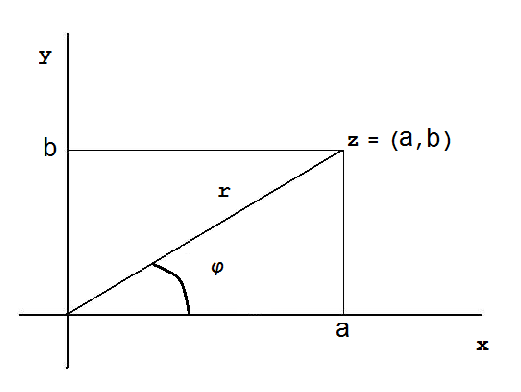
\epsfig{file=figura1.eps,clip=}
\vspace{-.4cm}
\end{center}
%\caption{Representaci{\'o} gr{\`a}fica del domini de la funci{\'o} $f(x)=\sqrt{1-x+y}$}
\end{figure}


\vspace{0.4cm}
\begin{definicio}
El nombre $\varphi$ tal que $\ 0\leq\varphi<2\pi\ $ s'anomena
\textbf{argument principal} de $z$ i es denota per $Arg\ z$.
(Tamb\'{e} se diu \textbf{valor principal} de $arg\ z$).
\end{definicio}

\vspace{0.4cm}
\begin{definicio}
Donat $z=(a,b)$ un nombre complex, $z\neq 0$ es pot
escriure com
$$z=|z|(\cos\varphi+i\sin\varphi)\,,$$
expressi{\'o}
coneguda com la \textbf{forma trigonom{\`e}trica} o \textbf{forma
polar} de $z$.
\end{definicio}

\vspace{0.4cm}
\notacio  A vegades tamb{\'e} s'utilitza la representaci{\'o}
m{\`o}dul argument $r_{\varphi}$.


\vspace{0.4cm}
\observacio  Si definim el conjunt d'arguments de $z$,
$$arg\;z=\{\theta\in \R\ :\ \theta=Arg\ z+2k\pi\ \ k\in \mathbb{Z} \}$$
llavors $z$ es pot escriure com:
$$z=|z|(\cos\theta+i\sin\theta)\hspace{0.5cm} \textrm{amb}\hspace{0.5cm} \theta\in arg\;z.$$

\vspace{0.4cm}
\begin{exemple}   Sigui $z=1+i\ $ aleshores, $\
|z|=\sqrt{1^{2}+1^{2}}=\sqrt2\ $ i
$\displaystyle\ Arg\ z=\arctan\frac{1}{1}=\frac{\pi}{4}$\\

d'on la forma trigonom{\`e}trica seria: $\displaystyle\quad
z=\sqrt2\left(\cos\frac{\pi}{4}+i\sin\frac{\pi}{4}\right)\,,$\\

i el conjunt d'arguments:$\quad arg\ z=\left\{\displaystyle\frac{\pi}{4}+2k\pi\ :\ k\in\ \mathbb{Z}\right\}\,.$\\
\end{exemple}

\begin{figure}[h!]
\begin{center}
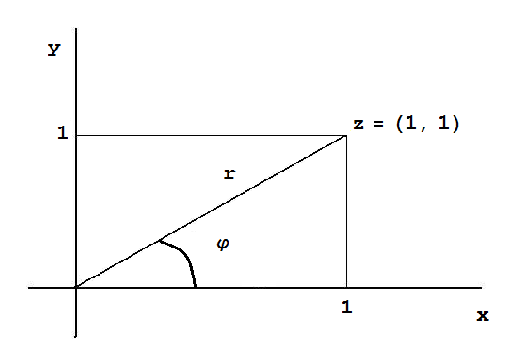
\epsfig{file=figura2.eps,clip=}
\vspace{-.4cm}
\end{center}
%\caption{Representaci{\'o} gr{\`a}fica del domini de la funci{\'o} $f(x)=\sqrt{1-x+y}$}
\end{figure}



\vspace{0.5cm}


\subsection{Operacions en la forma trigonom{\`e}trica}

\begin{center}
\textbf{Producte}
\end{center}


Siguin $z_{1},z_{2}\in \C\ $ tals que $\
z_{j}=|z_j|(\cos\theta_j+i\sin\theta_j)\,,\ \  \ \theta_j\in\
arg\ z_j\,,\ \ \ \ \ j=1,2.$\\

llavors\

\hspace{1.5cm}$z_1\cdot z_2=|z_1|(\cos\theta_1+i\sin\theta_1)\cdot
|z_2|(\cos\theta_2+i\sin\theta_2)=$\\

\hspace{1.5cm}$=
|z_1||z_2|((\cos\theta_1\cos\theta_2-\sin\theta_1\sin\theta_2)+i(\cos\theta_1\sin\theta_2+\cos\theta_2\sin\theta_1))=$\\

\hspace{1.5cm}$|z_1||z_2|(\cos(\theta_1+\theta_2)+i\sin(\theta_1+\theta_2))$\\

per tant: $\ \ \ |z_1\cdot z_2|=|z_1|\cdot|z_2|\ \ \ $      i   $\ \
\
\theta_1+\theta_2\in\ arg\ (z_1\cdot z_2)\,.$\\

\observacio Pel que hem dit abans dedu\"{\i}m que: si $\ z_1\cdot
z_2\neq0$\\

\hspace{1.5cm}$arg\ (z_1\cdot z_2)=arg\ z_1\ +\ arg\ z_2\ \ $
(igualtat entre conjunts).\\

\begin{center}
\textbf{Divisi{\'o}}
\end{center}

Siguin $\ \ z_1,z_2\in \C\ $\  amb\ $\ z_2\neq0\,,$ si deim $\ \
z=\displaystyle\frac{z_1}{z_2}=z_1\cdot\displaystyle\frac{1}{z_2}\ \
$ d'on $\ \ z_1=z\cdot
z_2\ \ $ i per les propietats del producte:\\

\hspace{2.5cm}$|z_1|=|z|\cdot|z_2|\Longrightarrow\
|z|=\displaystyle\frac{\ |z_1|\ }{|z_2|}$\

i tamb{\'e}

\hspace{1.5cm}$arg\ z_1=\ arg\ z+\ arg\ z_2\Longrightarrow\ arg\ z=\
arg\ z_1-\
arg\ z_2\ \ $ (igualtat entre conjunts).\\

\vspace{0.5cm}
D'aix{\`o} es dedueix f{\`a}cilment que

\vspace{0.5cm}
\hspace{1.5cm}si $z=r(\cos\ \varphi+i\sin\varphi)\ \ \ $ llavors $\
\ z^{-1}=\displaystyle\frac{1}{r}\left(\cos(-\varphi)+i\
\sin(-\varphi)\right).$

\newpage

\subsection{Forma exponencial d'un nombre complex}

L'equaci{\'o}

$$
 e^{i\theta}=\cos \theta+ i\ \sin\theta
$$

que defineix $\ e^{i\theta}\ $ per a tot $\ \theta\in \R\ $
s'anomena \textbf{f{\'o}rmula d'Euler}.\

Si escrivim un nombre complex no nul en forma polar
$z=r(\cos\theta+i\ \sin\theta),$ aleshores la f{\'o}rmula d'Euler
permet expressar $z$ m\'{e}s compactament en lo que s'anomena la
\textbf{forma exponencial}:

$$
z=r\,e^{i\theta}
$$

Les expressions del producte, divisi{\'o} i invers donades a la
secci{\'o} anterior se poden escriure de manera natural en forma
exponencial.\\

Siguin $\ z_1,z_2\neq0\ $ que venen donats per $\ z_1=r_1\
e^{i\theta_1}\,,\quad z_2=r_2\ e^{i\theta_2}\,,$ llavors:
\begin{center}
$z_1\cdot z_2=r_1 r_2\ e^{i(\theta_1+\theta_2)}$

\vspace{0.3cm} $\displaystyle\frac{z_1}{z_2}=\frac{r_1}{r_2}\
e^{i(\theta_1-\theta_2)}$

\vspace{0.3cm}$\displaystyle\frac{1}{z_1}=z^{-1}_1=\frac{1}{r_1}\
e^{-i\theta_1}$
\end{center}

\vspace{0.4cm}
\observacio Evidentment, donat $z\neq0,\ \ z\in \C$, t\'{e}
infinites expressions de la forma exponencial.
$$z=r\ e^{i(\theta+2k\pi)}\qquad k\in \mathbb{Z}\,.$$


\subsection{Pot{\`e}ncies i arrels}

\vspace{0.4cm}
\begin{definicio}
Donat $z\in \C\,,\ \ \ z\neq 0$, definim:

\hspace{1.5cm}$z^0=1\,.$

\hspace{1.5cm} $z^{n+1}=z^n\cdot z\,,\hspace{0.7cm} n\geq0\,,\ \ \
n\in \mathbb{Z}\,.$\

\hspace{1.5cm} $z^{-n}=(z^{-1})^n\,,\hspace{0.7cm} n\in \mathbb{N}.$
\end{definicio}

\vspace{0.4cm}
\begin{proposicio}

\begin{enumerate}

\item[a)] si $z=r\, e^{i\theta}\Longrightarrow z^{n}=r^{n}\, e^{in\theta}\,, \ \ \ n\in
\mathbb{Z}\,.$
\itemindent=1.5cm
    \item[b)] si $z\neq 0\,,\ \ \ \ \ z^n\cdot z^m=z^{n+m}\,, \ \ \ \ \ n,m\in \mathbb{Z}\,.$
    \item[c)] $(z_1\cdot z_2)^n=z_1^n\cdot z_2^n\,, \ \ \ \ \ n\in \mathbb{Z}\,.$
\end{enumerate}
\end{proposicio}


\vspace{0.4cm}
\observacio En el cas de $z\in \C$ tal que $|z|=1$, la propietat
$a)$ expressada en forma trigonom{\`e}trica queda:
$$(\cos\theta+i\sin\theta)^n=\cos{(n\theta)}+i\sin{(n\theta)}\,,\qquad n\in \mathbb{Z}\,,$$
que es coneix com \textbf{f{\'o}rmula de De Moivre}.\\

Per altra banda, si ens plantejam resoldre l'equaci{\'o} $\
w^n=z,\quad n\in \mathbb{N},\quad z\neq 0\,,$ \'{e}s a dir, trobar
les arrels n-{\`e}ssimes de $z$, tenim el  resultat seg{\"u}ent:

\begin{proposicio}
Tot $z\in \C-\{0\}$ admet $n$ arrels n-{\`e}ssimes diferents $\
w_0,w_1,...,w_{n-1}\,.$ Per calcular-les, si $|z|=r\ $ i $\ Arg\,
z=\varphi\ $ aleshores\\

\hspace{2.5cm} $|w_k|=\sqrt[n]{r}\,,\quad arg\,
 w_k=\displaystyle\frac{\varphi+2k\pi}{n},\qquad k=0,1,2,...,n-1\,.$
\end{proposicio}

%\demostracio
%Sigui $\ w=\rho\ e^{i\theta}\ $ tal que $\ w^n=z,\ $ llavors:\\
%
%$z=(\rho\ e^{i\theta})^n=\rho^n\ e^{in\theta}\ \  $ d'on $\
%\ \ |z|=r=\rho^n\ \  \Longrightarrow \ \ |w|=\rho=\sqrt[n]{r}\,.$\\
%
%$n\theta \in arg\ z \Longrightarrow \ \ n\theta=Arg\
%z+2k\pi=\varphi+2k\pi\ \ $ d'on $\ \
%\theta=\displaystyle\frac{\varphi+2k\pi}{n}\,, \ \
%k\in \mathbb{Z}.$\\
%
%Ara b\'{e}, nom\'{e}s quan $k=0,1,...,n-1\ $ tenim que corresponen a
%nombres complexos diferents.
%
%En efecte, si escrivim $\ \ \theta_k=\displaystyle\frac{\varphi+2 k
%\pi}{n}\,,\ \ k\in\Z\,,\ $ vegem que nom{\'e}s $\ \theta_0\,,\ldots
%\theta_{n-1}\ $
%representen a nombres complexos diferents.\\
%
%Donat $\ k\in \mathbb{Z}\,, \ \ k=n\, p+q\ $ amb $\ 0\leq q\leq
%n-1\,,\ $ llavors\\
%
%\hspace{1.5cm}$\theta_k=\displaystyle\frac{\varphi+2(n\,
%p+q)\pi}{n}=\displaystyle\frac{\varphi+2q\pi}{n}+2p\pi=\theta_q+2p\pi.$
%
%
%i per tant $\, \theta_k\,$ {\'e}s un argument que representa al mateix
%nombre que l'argument $\, \theta_q\,$. \hfill$\Box$\\

\vspace{0.4cm}
\observacio Si  miram els arguments de les  arrels n-{\`e}ssimes, veim que les difer{\`e}ncies dels arguments de
cada dues arrels consecutives s{\'o}n sempre iguals; concretament, totes valen
$\ {2\pi\over n}\,.$ Geom{\`e}tricament, aix{\`o} vol dir que les $n$ arrels n-{\`e}ssimes es troben sobre una
circumfer{\`e}ncia i formen els $n$ v{\`e}rtexs d'un pol{\'\i}gon regular de $n$ costats centrat a l'origen.\\


\vspace{0.4cm}
\begin{exemple}
 Resoleu l'equaci{\'o}: $\ z^4=-16$.
\end{exemple}

Com que $\ |-16|=16\ $ i $\ Arg\ (-16)=\pi$,
tenim que $\ |w_k|=\sqrt[4]{16}=2\ $ i que  $\ arg\
w_k=\frac{\pi+2k\pi}{4}\quad k=0,1,2,3.$

 Per tant, $\displaystyle\  Arg\ w_0=\frac{\pi}{4}\,,\quad Arg\ w_1=\frac{3\pi}{4}\,,\quad Arg\ w_2=\frac{5\pi}{4}\,,\quad Arg\ w_3=\frac{7\pi}{4}$


\begin{figure}[h!]
\begin{center}
%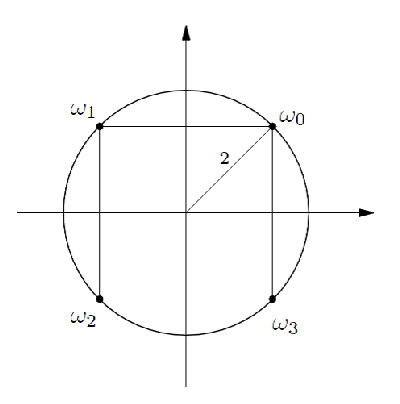
\epsfig{file=figura3.eps,clip=}
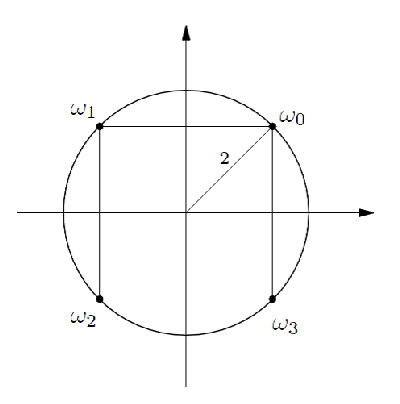
\includegraphics[width=5.5cm]{figura3.eps}
\vspace{-.4cm}
\end{center}
%\caption{Representaci{\'o} gr{\`a}fica del domini de la funci{\'o} $f(x)=\sqrt{1-x+y}$}
\end{figure}

\subsection{Exponencial d'un nombre complex}\label{exponencial}

\begin{definicio}
A tot nombre complex $z=a+bi$ s'associa un nou  nombre complex,
que anomenarem \textbf{exponencial de $z$} i indicarem per $e^z$,
definit per $$ e^z = e^a  (\cos b + i \sin b). $$
\end{definicio}

\vspace{0.4cm}\begin{observacio}
Si $z\in\R\ (Im\,  z=0$), aquesta definici{\'o} proporciona l'exponencial en $\R$.
\end{observacio}

\vspace{0.4cm}
\begin{proposicio}\label{propiexponencial}
Es compleixen les propietats seg{\"u}ents:
\item[a)] Si $z_1,z_2\in\C\,,$ aleshores $\ e^{z_1+z_2} = e^{z_1}\, e^{z_2}$
\item[b)] $e^z \not= 0\ $ per a tot $\ z\in\C$
\item[c)] $\displaystyle{1\over e^z}= e^{-z}\ $ per a tot $\ z\in\C$
\item[d)] Per a tot $b\in\R\,,\ e^{ib}= \cos b + i\sin b$
\item[e)] $\overline{e^{z}}=e^{\overline{z}}$
\item[f)] $\left| e^z\right| = e^a\,,$ on $z=a+bi$
\item[g)] $Arg \, e^z=b\, (\mbox{m{\`o}dul}\, 2\pi )$, on $z=a+bi$
\item[h)] $Re\, e^z = e^a\, \cos b\,,\quad Im\, e^z =e^a\, \sin b$
\end{proposicio}



\end{document}


